\documentclass[10pt]{beamer}

\usepackage{amssymb,amsmath}
\usepackage{graphicx}
\usepackage{url}
\usepackage{color}
\usepackage{pagenote}[continuous,page]
\usepackage{relsize}		% For \smaller
\usepackage{url}			% For \url
\usepackage{epstopdf}	% Included EPS files automatically converted to PDF to include with pdflatex

%For MindMaps
% \usepackage{tikz}%
% \usetikzlibrary{mindmap,trees,arrows}%

%%% Color Definitions %%%%%%%%%%%%%%%%%%%%%%%%%%%%%%%%%%%%%%%%%%%%%%%%%%%%%%%%%
%\definecolor{bordercol}{RGB}{40,40,40}
%\definecolor{headercol1}{RGB}{186,215,230}
%\definecolor{headercol2}{RGB}{80,80,80}
%\definecolor{headerfontcol}{RGB}{0,0,0}
%\definecolor{boxcolor}{RGB}{186,215,230}

%%% Save space in lists. Use this after the opening of the list %%%%%%%%%%%%%%%%
%\newcommand{\compresslist}{
%	\setlength{\itemsep}{1pt}
%	\setlength{\parskip}{0pt}
%	\setlength{\parsep}{0pt}
%}

%\setbeameroption{show notes on top}

% You should run 'pdflatex' TWICE, because of TOC issues.

% Rename this file.  A common temptation for first-time slide makers
% is to name it something like ``my_talk.tex'' or
% ``john_doe_talk.tex'' or even ``discrete_math_seminar_talk.tex''.
% You really won't like any of these titles the second time you give a
% talk.  Try naming your tex file something more descriptive, like
% ``riemann_hypothesis_short_proof_talk.tex''.  Even better (in case
% you recycle 99% of a talk, but still want to change a little, and
% retain copies of each), how about
% ``riemann_hypothesis_short_proof_MIT-Colloquium.2000-01-01.tex''?

\mode<presentation>
{
  \usetheme{CambridgeUS}
  \usecolortheme{dolphin}
  \useoutertheme{default}
  \useinnertheme{default}
  \setbeamercovered{invisible} % or whatever (possibly just delete it)
}
\beamertemplatenavigationsymbolsempty

\usepackage[english]{babel}
%\usepackage[latin1]{inputenc}
\usepackage{subfigure}

\usepackage{times}
\usepackage[T1]{fontenc}
\usepackage{CJKutf8}

%% makes the ppagenote command for figure references at the end.
\makepagenote
\renewcommand{\notenumintext}[1]{}
\newcommand{\ppagenote}[1]{\pagenote[Page \insertframenumber]{#1}}

\title[Experiment Design (01CH740)]{Experiment Design for Computer Sciences (01CH740)}
\author[Claus Aranha]{Claus Aranha\\{\footnotesize caranha@cs.tsukuba.ac.jp}}
\institute[U. Tsukuba]{University of Tsukuba, Department of Computer Sciences}



\title[]{Experiment Planning and Design}
\subtitle[]{Lecture 4: Statistical Concepts}
\author[Claus Aranha]{Claus Aranha\\{\footnotesize caranha@cs.tsukuba.ac.jp}}
\institute{Department of Computer Science}
\date{2015-05-12}

\begin{document}

\section{Outline}
\subsection{Outline}

\begin{frame}
  \maketitle
\end{frame}

\begin{frame}
  \frametitle{Notes} 
  \begin{itemize}
  \item Sorry about the sickness last class; Let's try Class 3 again!

    \bigskip

  \item No class on May 19th and May 26th;
  \end{itemize}
\end{frame}

\begin{frame}
  \frametitle{Class Outline}
  \begin{itemize}
  \item Random Variables
  \item Point Estimators
  \item Interval Estimators
  \item Hypothesis Testing
  \end{itemize}
  \begin{exampleblock}{}
    The goal of this class is to allow you to do a simple analysis of
    the data going into, and coming out of an experiment.
  \end{exampleblock}
\end{frame}

\section{Introduction}
\subsection{Introduction}
\begin{frame}
  \frametitle{Introduction: Probability vs Statistics}
  \begin{columns}
    \column{0.5\textwidth}
    \begin{block}{Probability}
      Given the pool, what are the odds of drawing a combination of certain colors?
      \begin{center}
      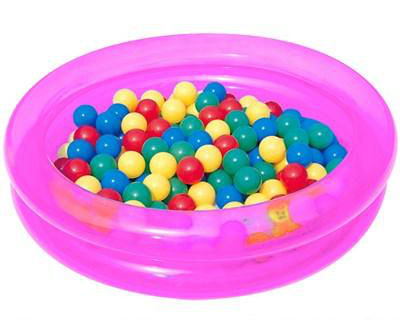
\includegraphics[height=.35\textheight]{img/ballpool}
      \end{center}
    \end{block}
    \column{0.5\textwidth}
    \begin{block}{Statistics}
      Given the colors of a few balls drawn, what can I know about the pool?
      \begin{center}
      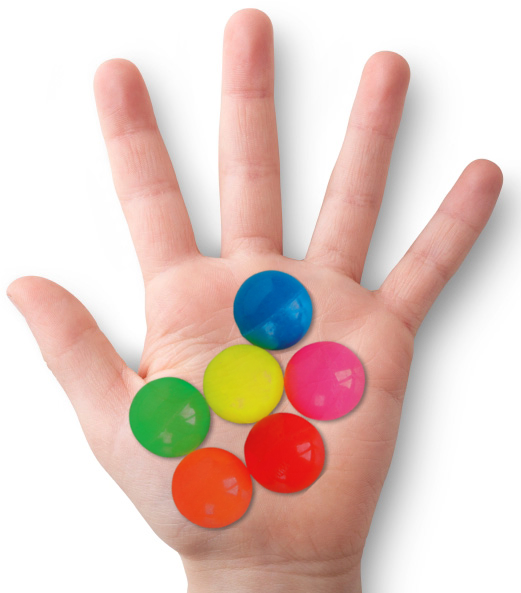
\includegraphics[height=.35\textheight]{img/ballhand}
      \end{center}
    \end{block}
  \end{columns}

  \bigskip

  \structure{Statistical Inference:} Using \emph{samples} to draw
  conclusions about \emph{populations}
\end{frame}

\begin{frame}
  \frametitle{Population, Sample and Observation}
  \begin{columns}
    \column{0.9\textwidth} ``A \structure{population} is a large set
    of objects of a similar nature which is of interest as a
    whole''. It can be an actual set (all balls in the pool), or an
    hypothetical one (all possible outcomes for an experiment).
    \column{0.1\textwidth}
    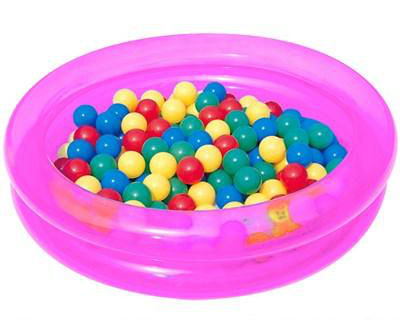
\includegraphics[width=1\textwidth]{img/ballpool}
  \end{columns}
  \vspace{.6cm}
  \begin{columns}
    \column{0.1\textwidth}
    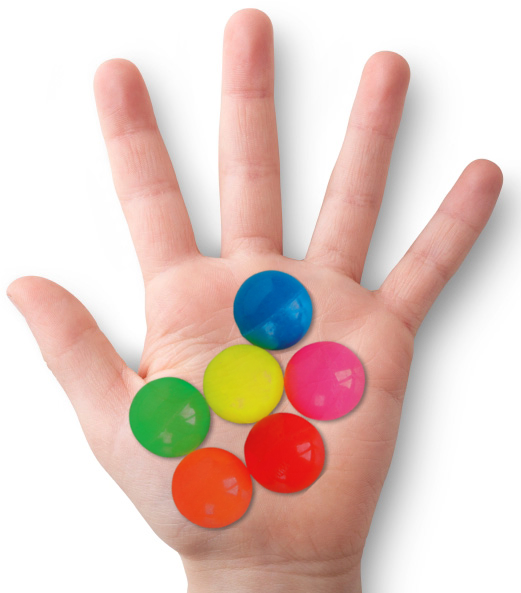
\includegraphics[width=1\textwidth]{img/ballhand}
    \column{0.9\textwidth} A \structure{sample} is a subset of a
    population. ``A sample is chosen to make inferences about the
    population by examining or measuring the elements in the sample''
  \end{columns}
  \vspace{.6cm}
  \begin{columns}
    \column{0.9\textwidth} An \structure{observation} is a single
      element of a given sample, an individual data point. An
      observation can also be considered as a sample of size one.
      \column{0.1\textwidth}
      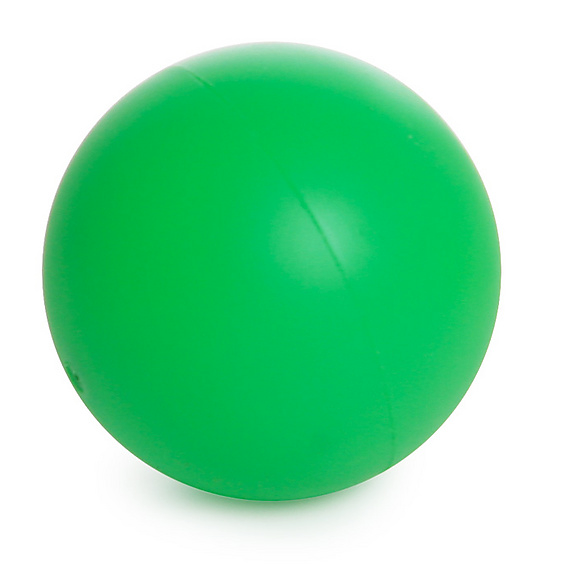
\includegraphics[width=1\textwidth]{img/greenball}
  \end{columns}

  \vspace{2cm}

  \rule{\textwidth}{0.4pt}
  \smaller{Glossary of statistical terms: \url{http://www.statistics.com/glossary}}
\end{frame}

\begin{frame}
  \frametitle{Population, Sample and Observation} 

  \begin{exampleblock}{Let's remember Alice and Bob's experiments}
    Alice and Bob build spam filter programs. They test their programs
    by counting how many spam the system catches in a day.
  \end{exampleblock}


  \begin{block}{Observation}
    \only<2>{
    If we count the number of spam caught by a system in one day, that
    is \structure{one observation}.

    \medskip
    
    If we count the number of spam caught by a system another day,
    that is \structure{a second observation}}
  \end{block}

  \begin{block}{Sample}
    
    \only<3>{If we count the number os spam caught every day for a
      week, we will have seven observations. That is a
      \structure{Sample}}
  \end{block}
  
  \begin{block}{Population}
    \only<4>{
      If we know ALL possible results for ALL possible days, that is the \structure{Population}
      
      \medskip
      
      In practice, it is \alert{usually impossible to KNOW} the
      population, but we want to learn \alert{as much as possible}
      from it, by observing samples.
    }
  \end{block}


\end{frame}

\section{Point and Interval Estimates}
\subsection{Concepts}

\begin{frame}
  \frametitle{Point and Interval Estimates} 

  Two central concepts of \structure{Statistical Inference} are
  \structure{point estimators} and \structure{statistical intervals}

  \medskip

  Both terms refer to the idea of using information obtained from a
  \structure{sample} to infer values about parameters of the
  \structure{population}.

  \vfill

  \begin{itemize}
    \item \structure{Point Estimate}: Estimate a value for a given population parameter
    \item \structure{Statistical Interval}: Estimate a interval of
      possible/probable values for a given population parameter;
  \end{itemize}
\end{frame}

\begin{frame}
  \frametitle{Point Estimates, Statistics, and Sampling distributions}
  
  Suppose one wants to obtain a point estimate for the mean of a given
  population. We take a sample of the population, and calculate the
  mean of that sample.

  \medskip

  However, a random sample from a population results in a random
  variable! Any function of the sample - any \emph{statistic} - is
  also a random variable.

  \medskip

  This means that statistics calculated from samples will also have
  their own probability distributions, called \structure{sampling
    distributions}.
  
  \begin{center}
    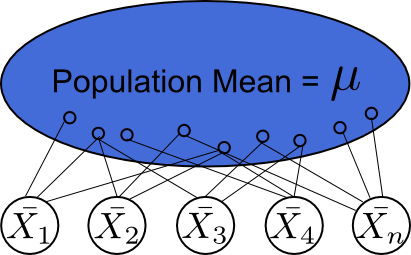
\includegraphics[width=0.3\textwidth]{img/meanestimator}
  \end{center}
  
  \rule{\textwidth}{0.4pt}
  {\tiny See D.W. Stockburger: \url{http://www.psychstat.missouristate.edu/introbook/sbk19.htm}}
\end{frame}

\begin{frame}[singleframe,fragile]
  \frametitle{I heard you like statistics!}
  {\small
  \begin{block}{}
    \begin{columns}
      
      \column{0.7\textwidth} 
      So in order to specify parameters of the population (such as
      means, deviation, etc), we draw a random sample and calculate the
      parameters from it.  
      \medskip

      But because the sample is random, the parameter calculated from
      the sample will also have its own statistics!
      \column{0.2\textwidth}
      
\includegraphics[width=.8\textwidth]{img/yodawg}      
    \end{columns}
  \end{block}
  \begin{exampleblock}{Everything is easier with an R example}
\begin{verbatim}
> population <- rnorm(100) # Pretend you don't know this!
> x1 <- sample(population,5)
> x2 <- sample(population,5)
> x3 <- sample(population,5)
> x1
[1]  0.6028260  0.1333065  1.1145946 -0.8675467 -0.4329469
> c(pop=mean(population),x1=mean(x1),x2=mean(x2),x3=mean(x3))
        pop          x1          x2          x3 
 0.05722922  0.11004669 -0.10459150  0.12630965
> c(mean(c(mean(x1),mean(x2),mean(x3))),sd(c(mean(x1),mean(x2),mean(x3))))
[1] 0.04392161 0.12887292
\end{verbatim}
  \end{exampleblock}
}
\end{frame}

\subsection{Point Estimators}
\begin{frame}
  \frametitle{Point Estimators}

  A \structure{Point Estimator} is a statistic which provides the
  value of maximum plausibility for a given (unknown) population
  parameter $\theta$.

  \medskip

  Consider a random variable $X$ distributed according to a given
  $f(X|\theta)$ (a population which distribution is controlled by this
  parameter)

  \medskip

  Now consider also a random sample from this variable:\\
  $x = \{x_1,x_2,\dots,x_N\}$;

  \medskip

  A given function $\hat{\Theta} = h(x)$ is called a \emph{point
    estimator} of the parameter $\theta$, and a value returned by this
  function for a given sample is referred to as a \emph{point estimate
    $\hat{\theta}$} of the parameter.
  
  \medskip

  \begin{block}{What does this mean?}
    A \structure{Point Estimator} is a function that, given a sample,
    generates an estimated parameter for the distribution from which
    the sample was obtained. 
  \end{block}

\end{frame}

\begin{frame}
  \frametitle{Point Estimators} 

  Point estimation problems arise frequently in all areas of science
  and engineering, whenever there is a need for estimating a parameter
  of a population:
  \begin{itemize}
    \item The population mean, $\mu$;
    \item The population variange, $\sigma^2$;
    \item a population proportion, $p$;
    \item the difference in the means of two populations, $\mu_1 - \mu_2$;
    \item etc...
  \end{itemize}

  For each cases (and many others) there are multiple ways of
  performing the estimation task. We choose the estimators based on
  its statistics.
  
  {\smaller
  \begin{exampleblock}{Multiple estimators?}
    We always consider only one definition for estimators (e.g., the
    mean). But we can be creative and invent others!

    \begin{equation*}
      \mu = \sum^N_{i=0}\frac{x_i}{N}
    \end{equation*}
    \begin{equation*}
      \mu' = \frac{max(x) - min(x)}{2}
    \end{equation*}
  \end{exampleblock}}
\end{frame}

\begin{frame}
  \frametitle{Evaluating Estimators} 

  A good estimator should consistently generate estimates that are
  close to the real value of the parameter $\theta$.

  \bigskip

  We say that an estimator $\hat{Theta}$ is \structure{unbiased} for a parameter $\theta$ if:
  \begin{equation*}
    E[\hat{\Theta}] = \theta
  \end{equation*}
  or, equivalently:
  \begin{equation*}
    E[\hat{\Theta}] - \theta = 0.
  \end{equation*}

  \bigskip

  The difference $E[\hat{\Theta}] - \theta$ is referred as the
  \structure{bias} of an estimator.

\end{frame}

\begin{frame}
  \frametitle{Evaluating Estimators}
  The usual estimators for mean and variance are unbiased estimators;

  Let $x_1,\dots,x_N$ be a random sample from a given population $X$,
  which is characterized by its mean $\mu$ and variance $\sigma^2$. In
  this situation, it is possible to show that:
  \begin{equation*}
    E[\bar{x}] = E[\frac{1}{N}\sum_{i = 1}^Nx_i] = \mu
  \end{equation*}
  and:
  \begin{equation*}
    E[s^2] = E[\frac{1}{N-1}\sum^N_{i=1}(x_i-\bar{x})^2] = \sigma^2
  \end{equation*}

  \vspace{2cm}

  \rule{\textwidth}{0.4pt}
  {\tiny See this link for an example proof:
    \url{http://isites.harvard.edu/fs/docs/icb.topic515975.files/Proof\%20that\%20Sample\%20Variance\%20is\%20Unbiased.pdf}}
\end{frame}

\begin{frame}
  \frametitle{Evaluating Estimators (2)} 

  There usually exists more than one unbiased estimator for a
  parameter $\theta$. One way to choose which to use is to select the
  one with the smallest variance. This is generally called the
  \emph{minimal-variance unbiased estimator} (MVUE).
  \begin{center}
    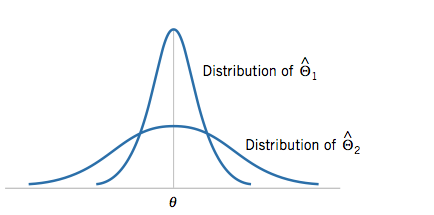
\includegraphics[width=.6\textwidth]{img/ubes-var}
  \end{center}
  MVUE have the ability of generating estimates $\hat{\theta}$ that
  are relatively close to the real value.
\end{frame}

% TODO: Think about adding slides 12-14 from campelo class 3 (or replace by an example?)

\subsection{The Central Limit Theorem}
\begin{frame}
  \frametitle{Distribution of samples} 

  Even for an arbitrary population, the sampling distribution of means
  tends to be approximately normal (with $E[\bar{x}] = \mu$ and $s_{\bar{x}} = \sigma^2/N$

  \vfill

  \begin{alertblock}{Warning! Maths!}
    More generally, let $x_1,\dots,x_n$ be a sequence of independent
    and identically distributed (\structure{iid}) random variables,
    with mean $\mu$ and finite variance $\sigma^2$. Then:
    \begin{equation*}
      z_n = \frac{\sum^n_{i=1}(x_i)-n\mu}{\sqrt{n\sigma^2}}
    \end{equation*}
    is distributed approximately as a standard normal variable. That is, $z_n ~ N(0,1)$
    
    \medskip
    
    This is the \structure{Central Limit Theorem}.
  \end{alertblock}
\end{frame}

\begin{frame}[singleslide,fragile]
  \frametitle{Example of the Central Limit Theorem}
  
  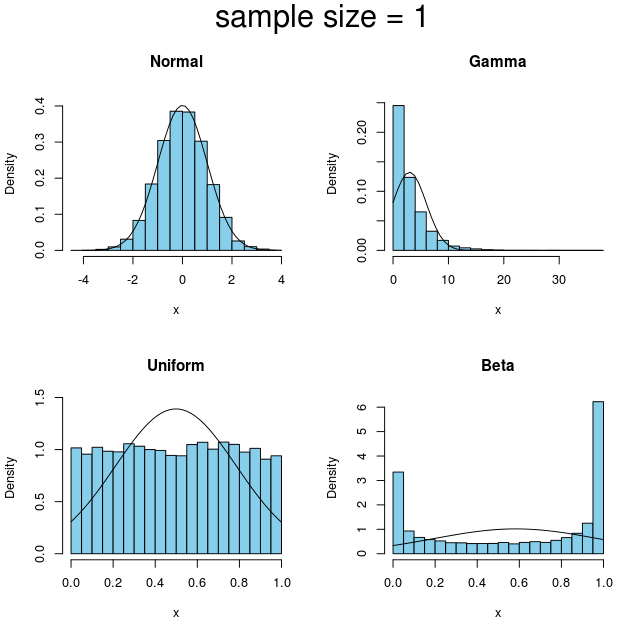
\includegraphics[width=.45\textwidth]{img/CLT1}\hfill
  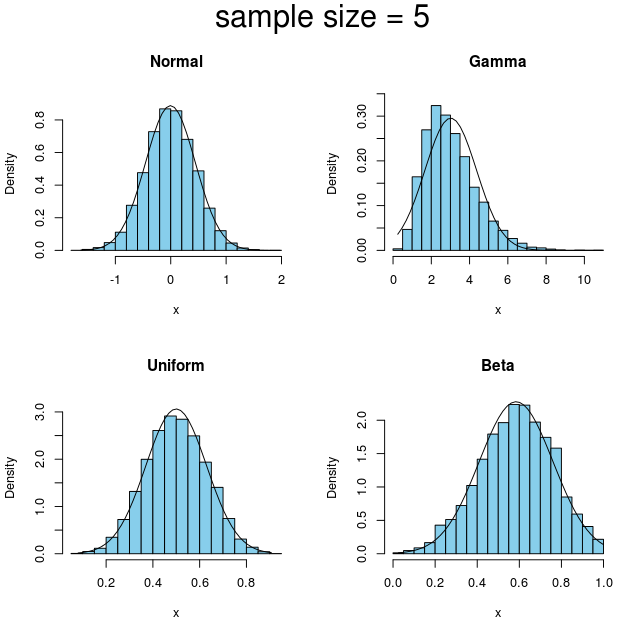
\includegraphics[width=.45\textwidth]{img/CLT5}

{\smaller
\begin{verbatim}
# Load the Teaching Demos library if you don't have it.
> install.packages("TeachingDemos")
> library(TeachingDemos)

> clt.examp()
> clt.examp(5)
\end{verbatim}}
\end{frame}

\begin{frame}
  \frametitle{Implications of the Central Limit Theorem} 

  The CLT is one of the most useful properties for statistical
  inference. The CLT allows the use of techniques based on the
  Gaussian distribution, even when the population under study is not
  normal.

  \bigskip
  
  For ``well-behaved'' distributions (continuous, symmetrical,
  unimodal) even small sample sizes are enough to justify invoking the
  CLT and using parametric techniques. 

  \bigskip

  For an interactive demonstration of the CLT, check:
  \url{http://drwho.cpdee.ufmg.br:3838/CLT/}
\end{frame}

% TODO: Add an example of point estimators

\begin{frame}
  \begin{center}
    mini-break, questions?
  \end{center}
\end{frame}


\section{Interval Estimators}
\section{Hypothesis Testing}
% TODO: Add campelo class 4
% TODO: Add campelo class 5

\section{End Notes}
\subsection{Homework 2}
\begin{frame}
  \frametitle{Homework 2}
  % Scatterplot of your data
  % Histogram of your data (which columns should you choose?)
  % Other plots that describe your data well

  % Do a hypothesis testing to compare different qualities of your data

  % OR
  % Provide some data that can be analysed and compared
\end{frame}

\section{Final Notes}
\subsection{Image Information}
\begin{frame}
  {\tiny
  \begin{itemize}
  \item Pool of balls image: \url{http://goo.gl/y8doaN}
  \item Green ball: \url{http://goo.gl/Fb8z68}
  \item MVUE image: D.C.Montgomery, G.C. Runger, ``Applied Statistics and Probability for Engineers'', Wiley 2003
  \end{itemize}
  }
  \medskip
  \begin{block}{This lecture notes is a derived work of}
    Felipe Campelo (2015), ``Lecture Notes on Design and Analysis of Experiments''\\
    Online: \url{https://github.com/fcampelo/Design-and-Analysis-of-Experiments}
    Creative Commons BY-NC-SA 4.0.
  \end{block}
\end{frame}

\end{document}
